\documentclass{article}
\usepackage[utf8]{inputenc}
\usepackage{amsmath}
\usepackage{amsfonts}
\usepackage{enumitem}
\usepackage{amssymb} 
\usepackage{xcolor}
\usepackage{soul}
\usepackage{todonotes}
\usepackage[margin=2.5cm]{geometry}
\graphicspath{ {./images/} }

\title{Graphs}
\author{Jin Long Cao, Qiaoru Zhang}
\date{December 2022}

\begin{document}
\maketitle
\section*{Weighted Function}
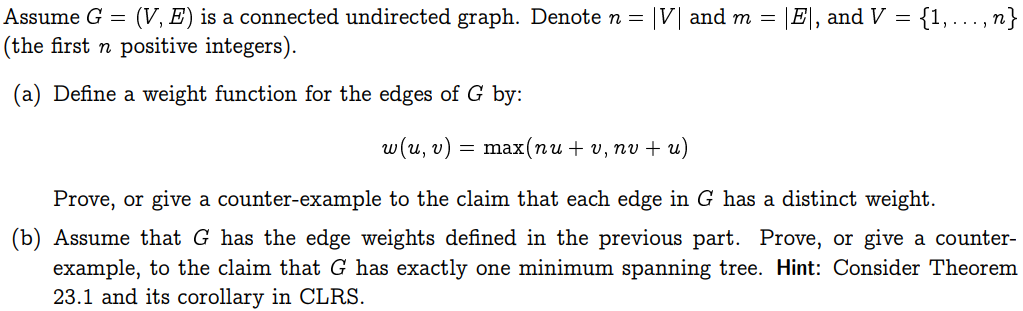
\includegraphics[width=\textwidth]{Weighted Function}
\section*{Solutions}
\subsection*{(a)} 
Suppose $G = (V, E)$ is a connected undirected graph. Denote $n = |V|$ and and $m = |E|$, and $V = \{1,\dots, n\}$ (the first $n$ positive integers).\\~\\
\underline{Proof by contradiction}: \\
Let $u_1,u_2,v_1,v_2 \in V$.\\
Assume $w(u_1, v_1) = w(u_2,v_2)$ such that $u_1 \neq u_2$ and $v_1 \neq v_2$ (Two different edges weight the same).\\
Without loss of generality, assume $u_1>v_1$ and $u_2>v_2$\\
Then, $w(u_1, v_1) = n \cdot u_1 + v_1$ and $w(u_2, v_2) = n \cdot u_2 + v_2$.\\
Now, we know $1 \leq v_1, v_2 < u_1,u_2 \leq n$\\
From our assumption and basic algebra, 
\begin{align*}
    w(u_1, v_1) &= w(u_2,v_2)\\
    n \cdot u_1 + v_1 & = n \cdot u_2 + v_2\\
    n \cdot u_1 - n \cdot u_2 &= v_2 - v_1\\
    n \cdot (u_1 - u_2) &= v_2 - v_1\\
    n &= \frac{v_2 - v_1}{u_1 - u_2}
\end{align*}
We conclude that $n = \frac{v_2 - v_1}{u_1 - u_2}$ but this is a contradiction since $v_2 - v_1 \leq n$ and the denominator cannot be a fraction since it is a difference of natural numbers (greater than 0). Hence our original assumption is false and we can conclude that each edge in $G$ has a distinct weight.

\subsection*{(b)} 
\underline{Theorem 23.1}: Let $G = (V, E)$ be a connected, undirected graph with a real-valued weight function $w$ defined on $E$. Let $A$ be a subset of $E$ that is included in some minimum spanning tree for $G$, let $(S, V-S)$ be any cut of $G$ that respects $A$, and let $(u,v)$ be a light edge crossing $(S, V-S)$. Then, edge $(u,v)$ is safe for $A$.\\~\\
\underline{Claim}: $G$ has exactly one minimum spanning tree\\
\underline{Proof}: \\
The light edge of $G$ would always be from vertex 1 to vertex 2 because each weight is dependent on the value of the vertex. \\
Let $A = \{(1,2)\} \subset E$, $S = \{$vertices in A$\}$, $V = \{1,\dots, n\}$. \\
Then $(S, V-S) = (\{1,2\},\{3,4,\dots, n\})$ is a cut of $G$ that respects $A$.\\ 
Notice that $\forall v_1 \in S, u_1 \in V-S$, $u>v$. \\
Therefore, $w(u_1,v_1) = n \cdot u_1 + v_1$ and the light edge that crosses $(S, V-S)$ will be $(u_2,v_2)$ where $v_2 = 1$ and $u_2 = \{$the smallest element in $V-S\}$ (by the definition of light edge).\\
Then by theorem 23.1, we know $(u_2, v_2)$ is safe for $A$ and would be added to $A$ such that $|A|$ and $|S|$ will increment by 1. Since each edge in $G$ has a distinct weight (from (a)), $(u_2, v_2)$ is unique.\\
This process will repeat until all vertices is added to $S$ and it will result the only possible minimum spanning tree $\{(1,2), (1,3), \dots, (1,n)\}$. Hence, $G$ has exactly one minimum spanning tree.
\section*{Minimum Spanning Tree}
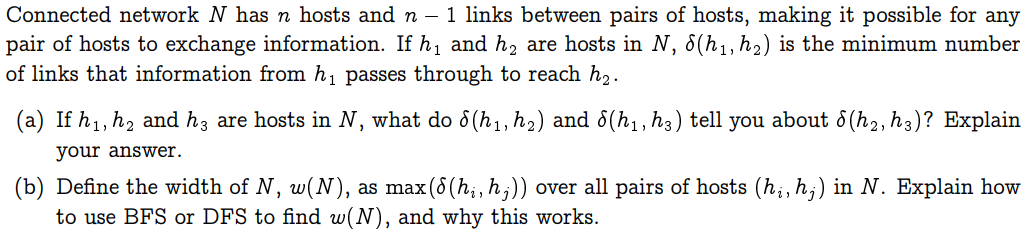
\includegraphics[width=\textwidth]{Minimum Spanning Tree}
\section*{Solutions}
Let $N$ be a connected network with $n$ hosts and $n-1$ links between pairs of host, making it possible for any pair of hosts to exchange information. If $h_1$ and $h_2$ are hosts in $N$, lets define $\delta(h_1, h_2)$ to be the minimum number of links that information from $h_1$ passes through to reach $h_2$.
\subsection*{(a)} 
Let $h_1, h_2$, and $h_3$ be hosts in $N$.\\
\underline{Claim}: $|\delta(h_1, h_2) - \delta(h_1, h_3)| \leq \delta(h_2, h_3) \leq \delta(h_1, h_2) + \delta(h_1, h_3)$\\~\\
\underline{Proof}:
Consider the three extreme cases,\\
\underline{Case 1}: The minimum path from $h_1$ to $h_2$ is completely different to the minimum path from $h_1$ to $h_3$. 
In other words, no links in the minimum path from $h_1$ to $h_2$ is also in the minimum path from $h_1$ to $h_3$. \\
Then we know $\delta(h_2, h_3) = \delta(h_1, h_2) + \delta(h_1, h_3)$ because the minimum path from $h_2$ to $h_3$ is the path $h_2$ to $h_1$ to $h_3$.\\
\underline{Case 2}: The minimum path from $h_1$ to $h_2$ $\subseteq$ the minimum path from $h_1$ to $h_3$. \\
In other words, every link in the minimum path from $h_1$ to $h_2$ is also in the minimum path from $h_1$ to $h_3$.\\
Then we know $\delta(h_2, h_3) = \delta(h_1, h_3) - \delta(h_1, h_2)$ because the minimum path from $h_1$ to $h_2$ overlaps with the minimum path from $h_1$ to $h_3$.\\
\underline{Case 3}: Similar to case 2 (vice versa of case 2). The minimum path from $h_1$ to $h_3$ $\subseteq$ the minimum path from $h_1$ to $h_2$. 
In other words, every link in the minimum path from $h_1$ to $h_3$ is also in the minimum path from $h_1$ to $h_2$.
Then we know $\delta(h_2, h_3) = \delta(h_1, h_2) - \delta(h_1, h_3)$ because the minimum path from $h_1$ to $h_3$ overlaps with the minimum path from $h_1$ to $h_2$.\\~\\
Now, the connected network $N$ we have is in between the three cases such that some (possibly all or none) links in one minimum path (say $h_1$ to $h_2$) is also in the other minimum path ($h_1$ to $h_3$) such that $|\delta(h_1, h_2) - \delta(h_1, h_3)| \leq \delta(h_2, h_3) \leq \delta(h_1, h_2) + \delta(h_1, h_3)$
\subsection*{(b)} 
Starting at any host in $N$, running BFS will give us a tree ($G_1$) with all the hosts (since it is a connected network). For each leaf in $G_1$, run a new BFS which will result in multiple different trees (lets call them $L_1, L_2, \dots, L_n$) for $n$ leaves. We run BFS on each leaf because they're the hosts farthest from our original starting host.\\
Now comparing the heights of $G_1$, $L_1, L_2, \dots$, and $L_n$. The greatest height is equal to the width of $N$.

\section*{Components Graph / Depth First Search}
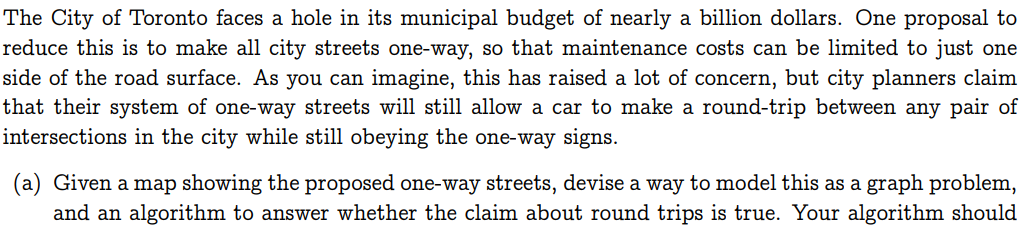
\includegraphics[width=\textwidth]{Components Graph1}
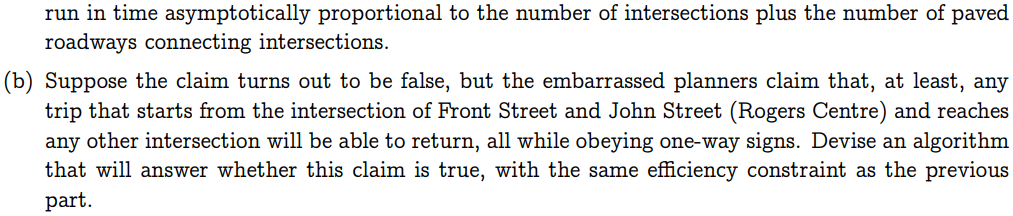
\includegraphics[width=\textwidth]{Components Graph2}
\section*{Solutions}
\subsection*{(a)} 
We will run DFS algorithm two times and using stack to solve this questions which required the total running time in O(V+E) time and we will imply the map into a strongly connected directed graph. The reason for using Stack to implement the algorithm is because we can do DFS traversal of complete graph and push every finished vertex to a stack, and by this way we could guarantee that the guarantee about the finished time will depend upon the sequence of vertices considered for DFS.\\

 % Let G = (V, E) be a directed graph, where V is the vertex set and E is the edge set. We assume the graph is represented as an adjacency structure, that is, for every vertex v there is a set adj(v) which is the set of vertices reachable by following one edge out of v. To do a depth first search we keep two pieces of information associated with each vertex v. One is the depth first search numbering num(v), and the other is mark(v), which indicates that v is currently on the recursion stack. This process examines all the edges and vertices. The call DFS(v) is made exactly once for each vertex in the graph. Each edge is placed into exactly one of four classes by the algorithm: tree edges, forward edges, cross edges and back edges.\\

\noindent And if we want to satisfied the claim, that one-way streets will still allow a car to make a round-trip between any pair of intersections, we can apply the the map into a strongly connected directed graph. Since a graph is said to be strongly connected if it has one strongly connected component. Which means the graph should be a cyclic graph, and we can check if is there a cycle if and only if the DFS algorithm will yields a back edge.\\

\noindent We will use the below graph G as an algorithm demonstration:\\


\begin{center}
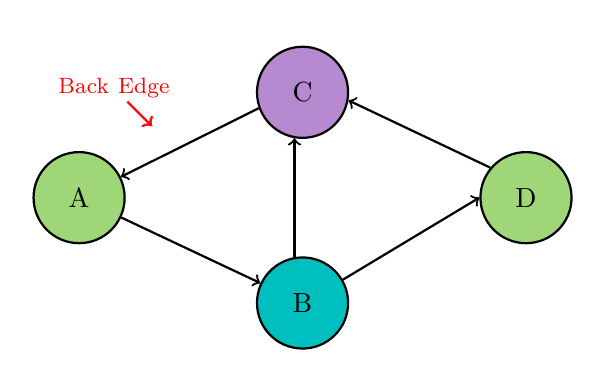
\begin{tikzpicture}[
circle,
    thick,
    box/.style={
        draw, 
        text width=1.5em, 
        align=center,
        minimum height=1cm
        fill=NodeFill,
        minimum size = 1.5em,
        inner sep= 6pt
    }
]
\begin{scope}[nodes=box, node distance=.5cm and 2cm]
\node (Anode) [fill={rgb:green,1;green,2;pink,5}]{A};
\draw (Anode.north) node[draw=none,above=7pt]{\hspace{-0.504cm} \textcolor{red}{\footnotesize \text{Back Edge}}}; 
\draw (Anode.north) node[draw=none,right=7pt]{\vspace{-0.8cm}\hspace{3.04cm}\textbf{\textcolor{red}{\pmb{$\searrow$}}}}; 

% \node (start) [left= 2cm of Anode, fill={rgb:yellow,1;yellow,2;pink,5}]  {start};
% \draw (start.north) node[draw=none,above=7pt]{\hspace{-0.504cm} \textcolor{red}{\footnotesize \text{Step 1}}}; 
% \draw (start.north) node[draw=none,above=-7pt]{\hspace{-0.4cm}\textbf{\textcolor{red}{\pmb{$\downarrow$}}}}; 


\node (end_node) [fill={rgb:blue,1;blue,1;pink,5},above right=of Anode] {C};
% \draw (end_node.north) node[draw=none,above=7pt]{\hspace{-0.504cm} \textcolor{red}{\footnotesize \text{Step 4, Step 6}}}; 
% \draw (end_node.north) node[draw=none,above=-7pt]{\hspace{-0.4cm}\textbf{\textcolor{red}{\pmb{$\downarrow$}}}}; 


\node (Bnode) [fill={rgb:pink,1;pink,1;pink,5},below right=of Anode] {B};
% \draw (Bnode.west) node[draw=none,above=-48pt]{\hspace{-0.90cm} \textcolor{red}{\footnotesize \text{Step 3}}}; 
% \draw (Bnode.west) node[draw=none,above=-35pt]{\hspace{-0.4cm}\textbf{\textcolor{red}{\pmb{$\nearrow$}}}}; 

\node (Dnode) [fill={rgb:green,1;green,2;pink,5},below right=of end_node] {D};
% \draw (Dnode.north) node[draw=none,above=7pt]{\hspace{-0.504cm} \textcolor{red}{\footnotesize \text{Step 4}}}; 
% \draw (Dnode.north) node[draw=none,above=-7pt]{\hspace{-0.4cm}\textbf{\textcolor{red}{\pmb{$\downarrow$}}}}; 

% \node (Cnode) [fill={rgb:green,1;green,2;pink,5},below = 1cm of Bnode]  {C};
% \draw (Cnode.west) node[draw=none,left=40pt]{\vspace{2cm} \textcolor{red}{\footnotesize \text{In scenario 1}}}; 
% \draw (Cnode.west) node[draw=none,left=30pt]{\vspace{3cm} \textcolor{red}{\footnotesize \text{Village C leads to an invalid path}}}; 
% \draw (Cnode.west) node[draw=none,left=30pt]{\vspace{4cm} \textcolor{red}{\footnotesize \text{since City B can only be passed once}}}; 
% \draw (Cnode.west) node[draw=none,above=-35pt]{\hspace{-0.4cm}\textbf{\textcolor{red}{\pmb{$\nearrow$}}}}; 
\end{scope}


\path [->] 
    % ([yshift=4mm]Anode.east) 
    %     edge node [above=1mm] {} 
    ([yshift=1.5mm]end_node.west);
% \path [->] 
%     ([yshift=-1.5mm]end_node.west) 
%         edge node [below=1mm] {} 
%     ([yshift=1mm]Anode.east);

\path [->]
      % (Anode.170) edge (start.10)
     % (start.345) edge (Anode.195)
    (Anode) edge (Bnode)
    % (Bnode.180) edge (Anode.310)
    (Bnode.30) edge (Dnode.180)
    % (Dnode.210) edge (Bnode.360)
    % (Bnode.280) edge (Cnode.80)
    % (Cnode.100) edge (Bnode.260)
    % (end_node.280) edge (Bnode.80)
    (Bnode.100) edge (end_node.260)
     (end_node.200) edge (Anode)
    (Dnode.140) edge (end_node.350);
\end{tikzpicture}
\end{center}

\noindent Suppose the graph G is strongly connected, to satisfy the claim in this question, then there will be one tree in the spanning forest root, and also there must be a way of getting from any vertex back to root vertex. If we want to find the strongly connected components in graph G:\\

% We could create an empty stack $S$ and apply DFS traversal of a graph. 
% we push the vertex to stack.
\noindent \textbf{Step 1}:  We could create an empty stack $S$ and apply DFS traversal of a graph. And apply DFS traversal of a graph. In the DFS traversal, after calling recursive DFS for adjacent vertices of a vertex, we will push the vertex to stack. This step will required the running time in O(V+E) time.\\

\noindent In the graph below, the path from vertex C to A will be Back Edge in the DFS algorithm (The red line indicate the Back Edge), hence we could know there exist a cycle path in the Graph G. Which can connect the start vertex A to vertex C through vertex B and D, and eventually back to vertex A. The strongly component is vertex A.

\begin{center}
\begin{tikzpicture}[
circle,
    thick,
    box/.style={
        draw, 
        text width=1.5em, 
        align=center,
        minimum height=1cm
        fill=NodeFill,
        minimum size = 1.5em,
        inner sep= 6pt
    }
]
\begin{scope}[nodes=box, node distance=.5cm and 2cm]
\node (Anode) [fill={rgb:green,1;green,2;pink,5}]{A};
\node (Bnode) [fill={rgb:pink,1;pink,1;pink,5}, right=of Anode] {B};
\node (Dnode) [fill={rgb:green,1;green,2;pink,5}, right=of Bnode] {D};
\node (end_node) [fill={rgb:blue,1;blue,1;pink,5}, right=of Dnode] {C};
\draw [->,red] (end_node.north) to [out=150,in=30] (Anode.north);

\end{scope}

\path [->]
    (Anode) edge (Bnode)
    (Bnode) edge (Dnode)
    (Dnode) edge (end_node)
\end{tikzpicture}
\end{center}

% \noindent \textbf{Step 2}: We will sort the dictionary $D$ by decreasing order according to the dictionary values. Which the last finished vertex will be the first item in the dictionary $D$. This step will required the running time in O(V) time.\\

\noindent \textbf{Step 2}: We will reverse the directions of all arrows to obtain the transpose graph. This step will required the running time in O(E) time.\\
\begin{center}
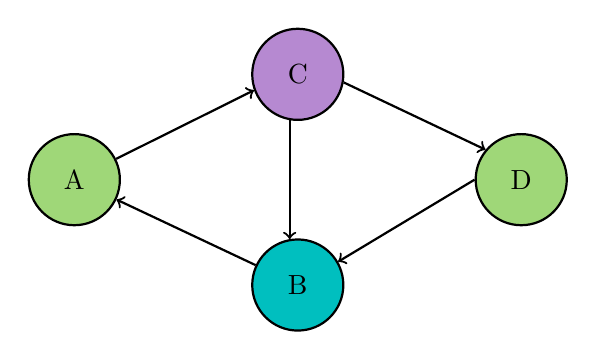
\begin{tikzpicture}[
circle,
    thick,
    box/.style={
        draw, 
        text width=1.5em, 
        align=center,
        minimum height=1cm
        fill=NodeFill,
        minimum size = 1.5em,
        inner sep= 6pt
    }
]
\begin{scope}[nodes=box, node distance=.5cm and 2cm]
\node (Anode) [fill={rgb:green,1;green,2;pink,5}]{A};
% \draw (Anode.north) node[draw=none,above=7pt]{\hspace{-0.504cm} \textcolor{red}{\footnotesize \text{Step 2}}}; 
% \draw (Anode.north) node[draw=none,above=-7pt]{\hspace{-0.4cm}\textbf{\textcolor{red}{\pmb{$\downarrow$}}}}; 

% \node (start) [left= 2cm of Anode, fill={rgb:yellow,1;yellow,2;pink,5}]  {start};
% \draw (start.north) node[draw=none,above=7pt]{\hspace{-0.504cm} \textcolor{red}{\footnotesize \text{Step 1}}}; 
% \draw (start.north) node[draw=none,above=-7pt]{\hspace{-0.4cm}\textbf{\textcolor{red}{\pmb{$\downarrow$}}}}; 


\node (end_node) [fill={rgb:blue,1;blue,1;pink,5},above right=of Anode] {C};
% \draw (end_node.north) node[draw=none,above=7pt]{\hspace{-0.504cm} \textcolor{red}{\footnotesize \text{Step 4, Step 6}}}; 
% \draw (end_node.north) node[draw=none,above=-7pt]{\hspace{-0.4cm}\textbf{\textcolor{red}{\pmb{$\downarrow$}}}}; 


\node (Bnode) [fill={rgb:pink,1;pink,1;pink,5},below right=of Anode] {B};
% \draw (Bnode.west) node[draw=none,above=-48pt]{\hspace{-0.90cm} \textcolor{red}{\footnotesize \text{Step 3}}}; 
% \draw (Bnode.west) node[draw=none,above=-35pt]{\hspace{-0.4cm}\textbf{\textcolor{red}{\pmb{$\nearrow$}}}}; 

\node (Dnode) [fill={rgb:green,1;green,2;pink,5},below right=of end_node] {D};
% \draw (Dnode.north) node[draw=none,above=7pt]{\hspace{-0.504cm} \textcolor{red}{\footnotesize \text{Step 4}}}; 
% \draw (Dnode.north) node[draw=none,above=-7pt]{\hspace{-0.4cm}\textbf{\textcolor{red}{\pmb{$\downarrow$}}}}; 

% \node (Cnode) [fill={rgb:green,1;green,2;pink,5},below = 1cm of Bnode]  {C};
% \draw (Cnode.west) node[draw=none,left=40pt]{\vspace{2cm} \textcolor{red}{\footnotesize \text{In scenario 1}}}; 
% \draw (Cnode.west) node[draw=none,left=30pt]{\vspace{3cm} \textcolor{red}{\footnotesize \text{Village C leads to an invalid path}}}; 
% \draw (Cnode.west) node[draw=none,left=30pt]{\vspace{4cm} \textcolor{red}{\footnotesize \text{since City B can only be passed once}}}; 
% \draw (Cnode.west) node[draw=none,above=-35pt]{\hspace{-0.4cm}\textbf{\textcolor{red}{\pmb{$\nearrow$}}}}; 
\end{scope}


\path [->] 
    % ([yshift=4mm]Anode.east) 
    %     edge node [above=1mm] {} 
    ([yshift=1.5mm]end_node.west);
% \path [->] 
%     ([yshift=-1.5mm]end_node.west) 
%         edge node [below=1mm] {} 
%     ([yshift=1mm]Anode.east);

\path [->]
      % (Anode.170) edge (start.10)
     % (start.345) edge (Anode.195)
    (Bnode) edge (Anode)
    % (Bnode.180) edge (Anode.310)
    (Dnode.180) edge (Bnode.30)
    % (Dnode.210) edge (Bnode.360)
    % (Bnode.280) edge (Cnode.80)
    % (Cnode.100) edge (Bnode.260)
    % (end_node.280) edge (Bnode.80)
    (end_node.260 ) edge (Bnode.100)
     (Anode) edge (end_node.200 )
    (end_node.350 ) edge (Dnode.140);
\end{tikzpicture}
\end{center}


\noindent \textbf{Step 3}: Then while the stack $S$ is not empty, we pop a vertex One by one from the stack. Let the popped vertex be ‘v’. And take v as source and do DFS again on the the transpose graph. The DFS starting from v prints strongly connected component of v. Which means each tree generated from the DFS forest is a strongly connected component. This step will required the running time in O(V+E) time.\\

\noindent In the graph below, the path from vertex A to C will be Back Edge in the DFS algorithm (The red line indicate the Back Edge), hence we could know there exist a cycle path in the Graph G. Which can connect the start vertex C to vertex A through  vertex D and B, and eventually back to vertex C. The strongly component is vertex C.

\begin{center}
\begin{tikzpicture}[
circle,
    thick,
    box/.style={
        draw, 
        text width=1.5em, 
        align=center,
        minimum height=1cm
        fill=NodeFill,
        minimum size = 1.5em,
        inner sep= 6pt
    }
]
\begin{scope}[nodes=box, node distance=.5cm and 2cm]
\node (Anode) [fill={rgb:green,1;green,2;pink,5}]{A};
\node (Bnode) [fill={rgb:pink,1;pink,1;pink,5}, right=of Anode] {B};
\node (Dnode) [fill={rgb:green,1;green,2;pink,5}, right=of Bnode] {D};
\node (end_node) [fill={rgb:blue,1;blue,1;pink,5}, right=of Dnode] {C};
\draw [->,red] (Anode.north) to [out=30,in=150] (end_node.north);

\end{scope}

\path [->]
    (Bnode) edge (Anode)
    (Dnode) edge (Bnode)
    (end_node) edge (Dnode)
\end{tikzpicture}
\end{center}
\\

\noindent Since we can observe that we can get the back edge by the DFS algorithm twice, it means that there is indeed a large cyclic graph that exists in this graph G. Also, we find that the first back edge is from C to A and the second one is from A to C. We find that their positions are actually interchanged. \\

\noindent The above algorithm is asymptotically optimal, since the above algorithm is based on DFS. It runs the DFS twice. if all vertices are reachable from the DFS starting point, then the DFS of the graph produces a tree, otherwise the DFS produces a forest. Thus the DFS of a graph with only one strongly connected component in our example graph G always produces a tree.\\

\noindent Therefore, we could conclude the total required running time for this algorithm is O(V+E), and we could find both the back edge and the strongly components, which means there exists a large cycle path in the Graph G which include all the vertex. Hence the claim "the system of one-way streets will still allow a car to make a round-trip between any pair of intersections in the city while still obeying the one-way signs." is true.\\
\subsection*{(b)} 
For this question, we will run DFS algorithm two times and using dictionary to solve this questions which required the total running time in O(V+E) time and we will imply the map into a strongly connected directed graph.\\

 % Let G = (V, E) be a directed graph, where V is the vertex set and E is the edge set. We assume the graph is represented as an adjacency structure, that is, for every vertex v there is a set adj(v) which is the set of vertices reachable by following one edge out of v. To do a depth first search we keep two pieces of information associated with each vertex v. One is the depth first search numbering num(v), and the other is mark(v), which indicates that v is currently on the recursion stack. This process examines all the edges and vertices. The call DFS(v) is made exactly once for each vertex in the graph. Each edge is placed into exactly one of four classes by the algorithm: tree edges, forward edges, cross edges and back edges.\\

\noindent And if we want to satisfied the claim, that one-way streets will still allow a car to make a round-trip between any pair of intersections, we can apply the the map into a strongly connected directed graph. Since the claim indicates "any trip that starts from the intersection of Front Street and John Street (Rogers Centre) and reaches any other intersection will be able to return, all while obeying one-way signs". Which means the graph should be one or more cyclic sub-graph in the graph G, and we can check if is there cycles if and only if the DFS algorithm will yields back edges.\\

\noindent We will use the below graph G as an algorithm demonstration:\\


\begin{center}
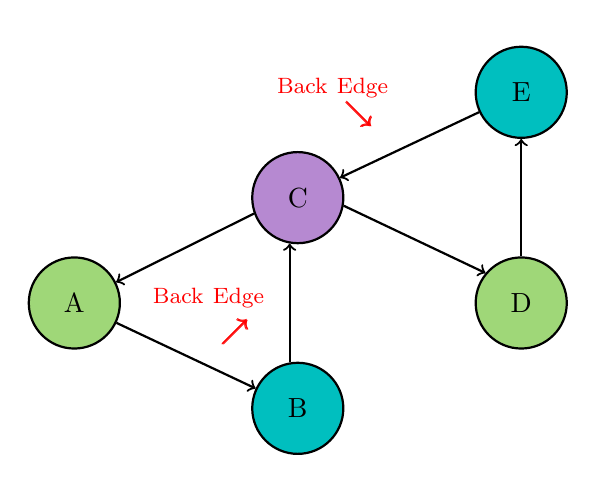
\begin{tikzpicture}[
circle,
    thick,
    box/.style={
        draw, 
        text width=1.5em, 
        align=center,
        minimum height=1cm
        fill=NodeFill,
        minimum size = 1.5em,
        inner sep= 6pt
    }
]
\begin{scope}[nodes=box, node distance=.5cm and 2cm]
\node (Anode) [fill={rgb:green,1;green,2;pink,5}]{A};
% \draw (Anode.north) node[draw=none,above=7pt]{\hspace{-0.504cm} \textcolor{red}{\footnotesize \text{Back Edge}}}; 
% \draw (Anode.north) node[draw=none,right=7pt]{\vspace{-0.8cm}\hspace{3.04cm}\textbf{\textcolor{red}{\pmb{$\searrow$}}}}; 

% \node (start) [left= 2cm of Anode, fill={rgb:yellow,1;yellow,2;pink,5}]  {start};
% \draw (start.north) node[draw=none,above=7pt]{\hspace{-0.504cm} \textcolor{red}{\footnotesize \text{Step 1}}}; 
% \draw (start.north) node[draw=none,above=-7pt]{\hspace{-0.4cm}\textbf{\textcolor{red}{\pmb{$\downarrow$}}}}; 


\node (end_node) [fill={rgb:blue,1;blue,1;pink,5},above right=of Anode] {C};
% \draw (end_node.north) node[draw=none,above=7pt]{\hspace{-0.504cm} \textcolor{red}{\footnotesize \text{Intersections}}}; 
% \draw (end_node.north) node[draw=none,above=-7pt]{\hspace{-0.4cm}\textbf{\textcolor{red}{\pmb{$\downarrow$}}}}; 
\draw (end_node.north) node[draw=none,above=7pt]{\hspace{-0.504cm} \textcolor{red}{\footnotesize \text{Back Edge}}}; 
\draw (end_node.north) node[draw=none,right=7pt]{\vspace{-0.8cm}\hspace{3.04cm}\textbf{\textcolor{red}{\pmb{$\searrow$}}}}; 

\node (Bnode) [fill={rgb:pink,1;pink,1;pink,5},below right=of Anode] {B};
\draw (Bnode.west) node[draw=none,above=23pt]{\hspace{-1.2cm} \textcolor{red}{\footnotesize \text{Back Edge}}}; 
\draw (Bnode.west) node[draw=none,above=10pt]{\hspace{-0.4cm}\textbf{\textcolor{red}{\pmb{$\nearrow$}}}}; 

\node (Enode) [fill={rgb:pink,1;pink,1;pink,5},above right=of end_node] {E};
% \draw (Bnode.west) node[draw=none,above=-48pt]{\hspace{-0.90cm} \textcolor{red}{\footnotesize \text{Step 3}}}; 
% \draw (Bnode.west) node[draw=none,above=-35pt]{\hspace{-0.4cm}\textbf{\textcolor{red}{\pmb{$\nearrow$}}}}; 

\node (Dnode) [fill={rgb:green,1;green,2;pink,5},below right=of end_node] {D};
% \draw (Dnode.north) node[draw=none,above=7pt]{\hspace{-0.504cm} \textcolor{red}{\footnotesize \text{Step 4}}}; 
% \draw (Dnode.north) node[draw=none,above=-7pt]{\hspace{-0.4cm}\textbf{\textcolor{red}{\pmb{$\downarrow$}}}}; 

% \node (Cnode) [fill={rgb:green,1;green,2;pink,5},below = 1cm of Bnode]  {C};
% \draw (Cnode.west) node[draw=none,left=40pt]{\vspace{2cm} \textcolor{red}{\footnotesize \text{In scenario 1}}}; 
% \draw (Cnode.west) node[draw=none,left=30pt]{\vspace{3cm} \textcolor{red}{\footnotesize \text{Village C leads to an invalid path}}}; 
% \draw (Cnode.west) node[draw=none,left=30pt]{\vspace{4cm} \textcolor{red}{\footnotesize \text{since City B can only be passed once}}}; 
% \draw (Cnode.west) node[draw=none,above=-35pt]{\hspace{-0.4cm}\textbf{\textcolor{red}{\pmb{$\nearrow$}}}}; 
\end{scope}


\path [->] 
    % ([yshift=4mm]Anode.east) 
    %     edge node [above=1mm] {} 
    ([yshift=1.5mm]end_node.west);
% \path [->] 
%     ([yshift=-1.5mm]end_node.west) 
%         edge node [below=1mm] {} 
%     ([yshift=1mm]Anode.east);

\path [->]
      % (Anode.170) edge (start.10)
     % (start.345) edge (Anode.195)
    (Anode) edge (Bnode)
    (Dnode) edge (Enode)
    (Enode) edge (end_node)
    % (Bnode.180) edge (Anode.310)
    % (Bnode.30) edge (Dnode.180)
    % (Dnode.210) edge (Bnode.360)
    % (Bnode.280) edge (Cnode.80)
    % (Cnode.100) edge (Bnode.260)
    % (end_node.280) edge (Bnode.80)
    (Bnode.100) edge (end_node.260)
     (end_node.200) edge (Anode)
    (end_node.350) edge (Dnode.140);
\end{tikzpicture}
\end{center}

\noindent Suppose the graph G is strongly connected, to satisfy the claim in this question, then there will be one tree in the spanning forest root, and also there must be a way of getting from any vertex back to root vertex. If we want to find the strongly connected components in graph G:\\

% We could create an empty stack $S$ and apply DFS traversal of a graph. 
% we push the vertex to stack.
\noindent \textbf{Step 1}:  We could create an empty dictionary $D$ and apply DFS traversal of a graph. In the DFS traversal, after calling recursive DFS for adjacent vertices of a vertex, we will append each vertex to the dictionary $D$, and each dictionary key is the vertex and the associate  value is the finish time f[v] for the vertex. This step will required the running time in O(V+E) time.\\

\noindent In the graph below, the path from vertex B to C will be Back Edge in the DFS algorithm (The red line indicate the Back Edge), hence we could know there exist a cycle path in the Graph G. Which can connect the start vertex C to vertex B through  vertex A, and eventually back to vertex C. \\

\noindent At the mean time, the path from vertex E to C will also be Back Edge in the DFS algorithm (The red line indicate the Back Edge), hence we could know there exist a cycle path in the Graph G. Which can connect the start vertex C to vertex B through  vertex D, and eventually back to vertex C. Hence there are two DFS tree exist in the graph G and the strongly component is vertex C.

\begin{center}
\begin{tikzpicture}[
circle,
    thick,
    box/.style={
        draw, 
        text width=1.5em, 
        align=center,
        minimum height=1cm
        fill=NodeFill,
        minimum size = 1.5em,
        inner sep= 6pt
    }
]
\begin{scope}[nodes=box, node distance=.5cm and 2cm]
% \node (Dnode) [fill={rgb:green,1;green,2;pink,5}, right=of Bnode] {D};
\node (end_node) [fill={rgb:blue,1;blue,1;pink,5}] {C};
\node (Anode) [fill={rgb:green,1;green,2;pink,5}, right=of end_node]{A};
\node (Bnode) [fill={rgb:pink,1;pink,1;pink,5}, right=of Anode] {B};
\draw [->,red] (Bnode.north) to [out=150,in=30] (end_node.north);

\end{scope}

\path [->]
    (end_node) edge (Anode)
    (Anode) edge (Bnode)
    % (Dnode) edge (end_node)
\end{tikzpicture}
\end{center}

\begin{center}
\begin{tikzpicture}[
circle,
    thick,
    box/.style={
        draw, 
        text width=1.5em, 
        align=center,
        minimum height=1cm
        fill=NodeFill,
        minimum size = 1.5em,
        inner sep= 6pt
    }
]
\begin{scope}[nodes=box, node distance=.5cm and 2cm]
% \node (Dnode) [fill={rgb:green,1;green,2;pink,5}, right=of Bnode] {D};
\node (end_node) [fill={rgb:blue,1;blue,1;pink,5}] {C};
\node (Anode) [fill={rgb:green,1;green,2;pink,5}, right=of end_node]{D};
\node (Bnode) [fill={rgb:pink,1;pink,1;pink,5}, right=of Anode] {E};
\draw [->,red] (Bnode.north) to [out=150,in=30] (end_node.north);

\end{scope}

\path [->]
    (end_node) edge (Anode)
    (Anode) edge (Bnode)
    % (Dnode) edge (end_node)
\end{tikzpicture}
\end{center}

\noindent \textbf{Step 2}: We will sort the dictionary $D$ by decreasing order according to the dictionary values. Which the last finished vertex will be the first item in the dictionary $D$. This step will required the running time in O(V) time.\\

\noindent \textbf{Step 3}: We will reverse the directions of all arrows to obtain the transpose graph. This step will required the running time in O(E) time.\\
\begin{center}
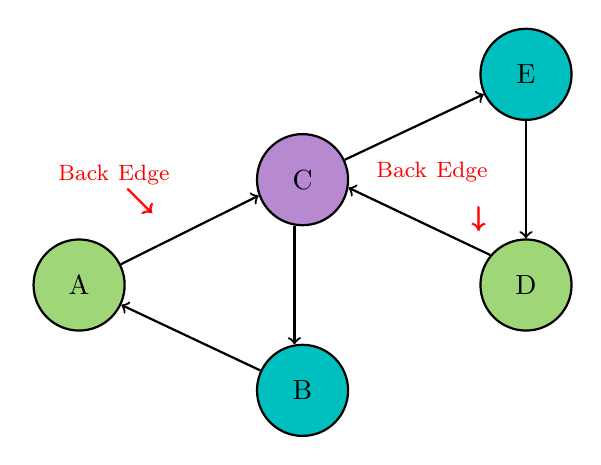
\begin{tikzpicture}[
circle,
    thick,
    box/.style={
        draw, 
        text width=1.5em, 
        align=center,
        minimum height=1cm
        fill=NodeFill,
        minimum size = 1.5em,
        inner sep= 6pt
    }
]
\begin{scope}[nodes=box, node distance=.5cm and 2cm]
\node (Anode) [fill={rgb:green,1;green,2;pink,5}]{A};
\draw (Anode.north) node[draw=none,above=7pt]{\hspace{-0.504cm} \textcolor{red}{\footnotesize \text{Back Edge}}}; 
\draw (Anode.north) node[draw=none,right=7pt]{\vspace{-0.8cm}\hspace{3.04cm}\textbf{\textcolor{red}{\pmb{$\searrow$}}}}; 

% \node (start) [left= 2cm of Anode, fill={rgb:yellow,1;yellow,2;pink,5}]  {start};
% \draw (start.north) node[draw=none,above=7pt]{\hspace{-0.504cm} \textcolor{red}{\footnotesize \text{Step 1}}}; 
% \draw (start.north) node[draw=none,above=-7pt]{\hspace{-0.4cm}\textbf{\textcolor{red}{\pmb{$\downarrow$}}}}; 


\node (end_node) [fill={rgb:blue,1;blue,1;pink,5},above right=of Anode] {C};
% \draw (end_node.north) node[draw=none,above=7pt]{\hspace{-0.504cm} \textcolor{red}{\footnotesize \text{Intersections}}}; 
% \draw (end_node.north) node[draw=none,above=-7pt]{\hspace{-0.4cm}\textbf{\textcolor{red}{\pmb{$\downarrow$}}}}; 
% \draw (end_node.north) node[draw=none,above=7pt]{\hspace{-0.504cm} \textcolor{red}{\footnotesize \text{Back Edge}}}; 
% \draw (end_node.north) node[draw=none,right=7pt]{\vspace{-0.8cm}\hspace{3.04cm}\textbf{\textcolor{red}{\pmb{$\searrow$}}}}; 

\node (Bnode) [fill={rgb:pink,1;pink,1;pink,5},below right=of Anode] {B};
% \draw (Bnode.west) node[draw=none,above=23pt]{\hspace{-1.2cm} \textcolor{red}{\footnotesize \text{Back Edge}}}; 
% \draw (Bnode.west) node[draw=none,above=10pt]{\hspace{-0.4cm}\textbf{\textcolor{red}{\pmb{$\nearrow$}}}}; 

\node (Enode) [fill={rgb:pink,1;pink,1;pink,5},above right=of end_node] {E};
% \draw (Bnode.west) node[draw=none,above=-48pt]{\hspace{-0.90cm} \textcolor{red}{\footnotesize \text{Step 3}}}; 
% \draw (Bnode.west) node[draw=none,above=-35pt]{\hspace{-0.4cm}\textbf{\textcolor{red}{\pmb{$\nearrow$}}}}; 

\node (Dnode) [fill={rgb:green,1;green,2;pink,5},below right=of end_node] {D};
\draw (Dnode.north) node[draw=none,above=7pt]{\hspace{-2.504cm} \textcolor{red}{\footnotesize \text{Back Edge}}}; 
\draw (Dnode.west) node[draw=none,above=7pt]{\hspace{-3.504cm} \textbf{\textcolor{red}{\pmb{$\downarrow$}}}}; 

% \node (Cnode) [fill={rgb:green,1;green,2;pink,5},below = 1cm of Bnode]  {C};
% \draw (Cnode.west) node[draw=none,left=40pt]{\vspace{2cm} \textcolor{red}{\footnotesize \text{In scenario 1}}}; 
% \draw (Cnode.west) node[draw=none,left=30pt]{\vspace{3cm} \textcolor{red}{\footnotesize \text{Village C leads to an invalid path}}}; 
% \draw (Cnode.west) node[draw=none,left=30pt]{\vspace{4cm} \textcolor{red}{\footnotesize \text{since City B can only be passed once}}}; 
% \draw (Cnode.west) node[draw=none,above=-35pt]{\hspace{-0.4cm}\textbf{\textcolor{red}{\pmb{$\nearrow$}}}}; 
\end{scope}


\path [->] 
    % ([yshift=4mm]Anode.east) 
    %     edge node [above=1mm] {} 
    ([yshift=1.5mm]end_node.west);
% \path [->] 
%     ([yshift=-1.5mm]end_node.west) 
%         edge node [below=1mm] {} 
%     ([yshift=1mm]Anode.east);

\path [->]
      % (Anode.170) edge (start.10)
     % (start.345) edge (Anode.195)
    ( Bnode) edge (Anode)
    ( Enode) edge (Dnode)
    ( end_node) edge (Enode)
    % (Bnode.180) edge (Anode.310)
    % (Bnode.30) edge (Dnode.180)
    % (Dnode.210) edge (Bnode.360)
    % (Bnode.280) edge (Cnode.80)
    % (Cnode.100) edge (Bnode.260)
    % (end_node.280) edge (Bnode.80)
    ( end_node.260) edge (Bnode.100)
     ( Anode) edge (end_node.200)
    (Dnode.140) edge (end_node.350 );
\end{tikzpicture}
\end{center}


\noindent \textbf{Step 4}: Then while the dictionary is not empty, we pop a vertex One by one from dictionary $D$ from the first index. Let the popped vertex be ‘v’. And take v as source and do DFS again on the the transpose graph. The DFS starting from v prints strongly connected component of v. Which means each tree generated from the DFS forest is a strongly connected component. This step will required the running time in O(V+E) time.\\

\noindent In the graph below, the path from vertex A to C will be Back Edge in the DFS algorithm (The red line indicate the Back Edge), hence we could know there exist a cycle path in the Graph G. Which can connect the start vertex C to vertex a through  vertex B, and eventually back to vertex C. \\

\noindent At the mean time, the path from vertex D to C will also be Back Edge in the DFS algorithm (The red line indicate the Back Edge), hence we could know there exist a cycle path in the Graph G. Which can connect the start vertex C to vertex D through vertex E, and eventually back to vertex C. Hence there are two DFS tree exist in the graph G and the strongly component is vertex C.

\begin{center}
\begin{tikzpicture}[
circle,
    thick,
    box/.style={
        draw, 
        text width=1.5em, 
        align=center,
        minimum height=1cm
        fill=NodeFill,
        minimum size = 1.5em,
        inner sep= 6pt
    }
]
\begin{scope}[nodes=box, node distance=.5cm and 2cm]
% \node (Dnode) [fill={rgb:green,1;green,2;pink,5}, right=of Bnode] {D};
\node (end_node) [fill={rgb:blue,1;blue,1;pink,5}] {C};
\node (Bnode) [fill={rgb:pink,1;pink,1;pink,5}, right=of end_node] {B};
\node (Anode) [fill={rgb:green,1;green,2;pink,5}, right=of Bnode]{A};
\draw [->,red] (Anode.north) to [out=150,in=30] (end_node.north);

\end{scope}

\path [->]
    (end_node) edge (Bnode)
    (Bnode) edge (Anode)
    % (Dnode) edge (end_node)
\end{tikzpicture}
\end{center}

\begin{center}
\begin{tikzpicture}[
circle,
    thick,
    box/.style={
        draw, 
        text width=1.5em, 
        align=center,
        minimum height=1cm
        fill=NodeFill,
        minimum size = 1.5em,
        inner sep= 6pt
    }
]
\begin{scope}[nodes=box, node distance=.5cm and 2cm]
% \node (Dnode) [fill={rgb:green,1;green,2;pink,5}, right=of Bnode] {D};
\node (end_node) [fill={rgb:blue,1;blue,1;pink,5}] {C};
\node (Bnode) [fill={rgb:pink,1;pink,1;pink,5}, right=of end_node] {E};
\node (Anode) [fill={rgb:green,1;green,2;pink,5}, right=of Bnode]{D};
\draw [->,red] (Anode.north) to [out=150,in=30] (end_node.north);

\end{scope}

\path [->]
    (end_node) edge (Bnode)
    (Bnode) edge (Anode)
    % (Dnode) edge (end_node)
\end{tikzpicture}
\end{center}

\noindent Since we can observe that we can get the back edges by the DFS algorithm twice, it means that there is indeed two large cyclic sub-graph that exists in this graph G. Also, we find that the first back edge is (B - C and E - C) and the second one is (A - C and D - C). We could observe that C is the strongly component for both of the sub-trees. \\

\noindent Therefore, the above algorithm is asymptotically optimal, since the above algorithm is based on DFS. It runs the DFS twice. if all vertices are reachable from the DFS starting point, then the DFS of the graph could also produces two sub DFS trees. Thus the DFS of a graph with only one strongly connected component in our example graph G could always produces forests.\\

\noindent Therefore, we could conclude the total required running time for this algorithm is O(V+E), and we could find both the back edges and the strongly component, which means there exists two large cycle paths in the Graph G which include all the vertex. Hence the claim "any trip that starts from the intersection of Front Street and John Street (Rogers Centre) and reaches any other intersection will be able to return, all while obeying one-way signs" is true.\\
\newpage
\section*{Colourable / Breadth First Search}
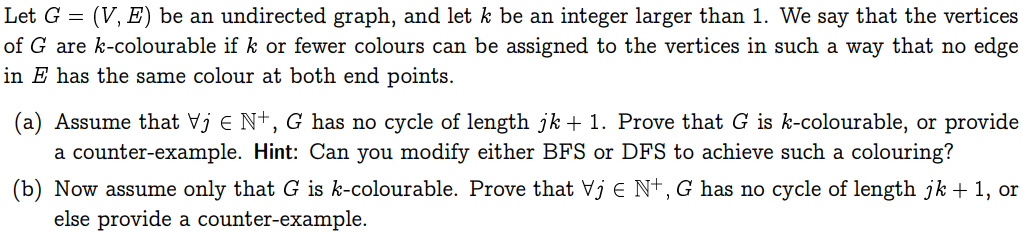
\includegraphics[width=\textwidth]{Colourable}
\section*{Solutions}
\subsubsection*{(a)} 
We will use an updated version of the BFS method to implement this question, colouring each node from 1 to n green and begin BFS traversal from the starting node that has not yet been visited to simultaneously cover all connected components. When the BFS traversal reaches a node, we will perform the following actions: (1) we check all of the tree edges of the current node; (2) for each vertex connected to the current node via the tree edge, we check if the colours of the nodes are the same; if they are, we change the color of the other nodes; and we check whether the node has been visited before; if so, we mark it as a visited node and push it into a queue. (3) we check if the total number of colors exsits in the graph exceed K or not, if it exceeds, we return False; (4) Once we finish visiting all the nodes, return true.\\~\\
Since given an undirected and connected graph, $\forall j \in N^+$ a cycle of length $jk + 1$ simply means that the cycle contains ($jk + 1$) vertices and ($jk + 1$) edges. And since for an undirected graph, the degree of a node is the number of edges incident to it. Hence if we know that there is no cycle of length in the graph is equal to ($jk + 1$), then we could assume the maximum weight of the graph (the number of edges and nodes incident to a node in the graph) is $jk$.\\

\noindent We will prove by using induction on the number of vertices in the graph, which we denote by n. Let P(n) be the proposition that an n-vertex graph with maximum degree at most $jk$ is $k$-colorable.\\~\\
\underline{Base Case}: when k = 2:\\
Since k is larger than 1, hence the smallest value of k could be 2, and $j \in N^+$, hence the smallest value of j could be 1. \\
\underline{Case 1}: When j = 1:\\
Example graph:
\begin{center}
\begin{tikzpicture}[
circle,
    thick,
    box/.style={
        draw, 
        text width=1.5em, 
        align=center,
        minimum height=1cm
        fill=NodeFill,
        minimum size = 1.5em,
        inner sep= 6pt
    }
]
\begin{scope}[nodes=box, node distance=.5cm and 2cm]
\node (Anode) [fill={rgb:green,1;green,2;pink,5}]{A};
\node (end_node) [fill={rgb:pink,1;pink,1;pink,5},below left=of Anode] {B};
\node (Bnode) [fill={rgb:pink,1;pink,1;pink,5},below right=of Anode] {C};
\node (Dnode) [fill={rgb:green,1;green,2;pink,5},below right=of end_node] {E};
\node (Enode) [fill={rgb:green,1;green,2;pink,5},below left=of end_node] {D};
% \node (Fnode) [fill={rgb:green,1;green,2;pink,5},below right=of Bnode] {F};
% \node (Gnode) [fill={rgb:green,1;green,2;pink,5},below left=of Bnode] {G};
\end{scope}


\path [-]
    %   % (Anode.170) edge (start.10)
    %  % (start.345) edge (Anode.195)
    (Anode) edge (end_node)
    (Anode) edge (Bnode)
    (end_node) edge (Enode)
    (end_node) edge (Dnode)
    % % (Bnode.180) edge (Anode.310)
    % (Bnode.30) edge (Dnode.180)
    % % (Dnode.210) edge (Bnode.360)
    % % (Bnode.280) edge (Cnode.80)
    % % (Cnode.100) edge (Bnode.260)
    % % (end_node.280) edge (Bnode.80)
    % (Bnode.100) edge (end_node.260)
    %  (end_node.200) edge (Anode)
    % (Dnode.140) edge (end_node.350);
\end{tikzpicture}
\end{center}
\\

\noindent Therefore the smallest value of $jk$ could be 2. When $jk$ = 2, which means for some node exists in the graph, it's maximum degree is 2. Which means there exists 2 sub-childs for each nodes in the graph. Also since G is a undirected graph, to avoid no edge should have two vertices of the same color. As shown in the graph above, each vertex's color is different with its sub-child, and each weight of vertex is 2. Hence we could observe that there exist 2 color in the graph, which is 2-colorable graph. Hence p(n) holds.\\~\\
\underline{Case 2}: When j $>$ 1:\\
Example graph:
\begin{center}
\begin{tikzpicture}[
circle,
    thick,
    box/.style={
        draw, 
        text width=1.5em, 
        align=center,
        minimum height=1cm
        fill=NodeFill,
        minimum size = 1em,
        inner sep= 1pt
    }
]
\begin{scope}[nodes=box, node distance=.5cm and 2cm]
\node (Anode) [fill={rgb:green,1;green,2;pink,5}]{A};
\node (Bnode) [fill={rgb:pink,1;pink,1;pink,5},below right=of Anode] {B};
\node (Cnode) [fill={rgb:green,1;green,2;pink,5},below left=of Bnode] {C};
\node (Dnode) [fill={rgb:pink,1;pink,1;pink,5},below right=of Cnode] {D};
\node (Enode) [fill={rgb:green,1;green,2;pink,5},below left=of Dnode] {E};
\node (Fnode) [fill={rgb:pink,1;pink,1;pink,5},below right=of Enode] {F};
\node (Gnode) [fill={rgb:green,1;green,2;pink,5},below left=of Fnode] {G};
\node (Hnode) [fill={rgb:pink,1;pink,1;pink,5},below right=of Gnode] {H};
\node (Inode) [fill={rgb:green,1;green,2;pink,5},below left=of Hnode] {I};
\end{scope}

\path [-]
    (Anode) edge (Bnode)
    (Anode) edge (Dnode)
    (Anode) edge (Fnode)
    (Anode) edge (Hnode)
    (Cnode) edge (Bnode)
    (Cnode) edge (Dnode)
    (Cnode) edge (Fnode)
    (Cnode) edge (Hnode)
    (Enode) edge (Bnode)
    (Enode) edge (Dnode)
    (Enode) edge (Fnode)
    (Enode) edge (Hnode)
    (Gnode) edge (Bnode)
    (Gnode) edge (Dnode)
    (Gnode) edge (Fnode)
    (Gnode) edge (Hnode)
    (Inode) edge (Bnode)
    (Inode) edge (Dnode)
    (Inode) edge (Fnode)
    (Inode) edge (Hnode)
\end{tikzpicture}
\end{center}

\noindent Suppose we pick any vertex A from the provided tree T. Let T be a tree with roots at vertex A. Assume the root A is given the first colour. Paint the second colour on all the vertices that are close to A. The adjacent vertices in the third floor should then be painted with the first colour. Continue doing this until all of T's vertices are painted. Thus, any vertex that is distant from A by an odd number has a second colour. While the first colour belongs to v and vertices that are evenly spaced from v. Hence there need at least ($k$) = 2 colors required in the graph. As shown in the graph above, each vertex's color is different with its sub-child, and each weight of vertex $\geq$ 2. Hence we could observe that there exist 2 color in the graph, which is 2-colorable graph. Hence p(n) holds.\\

\noindent Inductive steps: k $>$ 2:

\noindent If we assume that P(n) is true, and let G be an (n + 1) vertex graph with maximum degree at most $jk$. Remove a vertex v (and all edges incident to it), leaving an n-vertex subgraph, H. The maximum degree of H is at most $jk$, and so H is ($k$+ 1)-colorable by our assumption P(n). Now add back vertex v. We can assign v a color (from the set of $k$ + 1 colors) that is different from all its adjacent vertices, since there are at most $jk$ vertices adjacent to v and so at least one of the $k$ + 1 colors is still available. Therefore, G is ($k$ + 1)-colorable. Hence we could proved the theorem follows by induction.\\


\subsubsection*{(b)} 
Counter-example graph:
\begin{center}
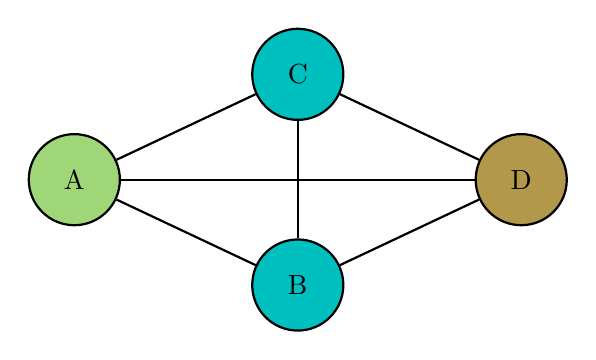
\begin{tikzpicture}[
circle,
    thick,
    box/.style={
        draw, 
        text width=1.5em, 
        align=center,
        minimum height=1cm
        fill=NodeFill,
        minimum size = 1.5em,
        inner sep= 6pt
    }
]
\begin{scope}[nodes=box, node distance=.5cm and 2cm]
\node (Anode) [fill={rgb:green,1;green,2;pink,5}]{A};
\node (end_node) [fill={rgb:pink,;pink,1;pink,5},above right=of Anode] {C};
\node (Bnode) [fill={rgb:pink,1;pink,1;pink,5},below right=of Anode] {B};
% \node (Enode) [fill={rgb:green,1;green,2;pink,5}, below right=of Bnode] {E};
\node (Dnode) [fill={rgb:red,4;green,4;pink,5},below right=of end_node] {D};
\end{scope}


\path [-] 
    % ([yshift=4mm]Anode.east) 
    %     edge node [above=1mm] {} 
    ([yshift=1.5mm]end_node.west);
% \path [->] 
%     ([yshift=-1.5mm]end_node.west) 
%         edge node [below=1mm] {} 
%     ([yshift=1mm]Anode.east);

\path [-]
      % (Anode.170) edge (start.10)
     % (start.345) edge (Anode.195)
    (Anode) edge (Bnode)
    (Anode) edge (Dnode)
    % (Bnode) edge (Enode)
    % (Bnode.180) edge (Anode.310)
    (Bnode) edge (Dnode)
    % (Dnode.210) edge (Bnode.360)
    % (Bnode.280) edge (Cnode.80)
    % (Cnode.100) edge (Bnode.260)
    % (end_node.280) edge (Bnode.80)
    (Bnode) edge (end_node)
     (end_node) edge (Anode)
    (Dnode) edge (end_node);
\end{tikzpicture}
\end{center}

\noindent As the counter-example graph shown above, this graph is a 3-colourable graph, where K = 3. However, when j = 1, the graph G has a cycle $\{(A,B), (B,D), (D,C), (C,A)\}$ of length of 4, which includes (A - B, B - D, D - C, C - A) four paths  and ( A , B , C , D) 4 nodes. In this case the $jk = 3$, $jk + 1 = 3 = 1 = 4$. Hence this graph G is 3-colourable, which j =1, $j \in N^+$. And G has a cycle of length $jk + 1 = 4$, which violates the assumption.

% We will prove by using induction on the number of vertices in the graph, which we denote by n. Let P(n) be the proposition that an n-vertex graph G, when G is $k-colourable$, $\forall j \in N^+$, with maximum degree of the graph G is most $jk$.\\

% \noindent Base Case:

% \noindent When $j = 1$: Suppose the graph is 3-colorable, hence we could know that ($jk$ + 1) = 2 + 1 = 3, where $jk$ = 2, which means for some node exists in the graph, it's maximum degree is 2, which means there at least exists 3 nodes in the graph. Also since G is a undirected graph, to avoid no edge should have two vertices of the same color. Hence there need at least ($jk$ + 1) = 2 + 1 = 3 colors required in the graph. Hence P(n) holds when \\

% \noindent Inductive steps:

% \noindent When $j > 1$: If we assume that P(n) is true, and let G be an (n + 1) vertex graph with maximum degree at most $jk$. Remove a vertex v (and all edges incident to it), leaving an n-vertex subgraph, H. The H is ($k$+ 1)-colorable, so maximum degree of H is at most $jk$  by our assumption P(n). Now add back vertex v. We can assign v a color (from the set of $k$ + 1 colors) that is different from all its adjacent vertices, since there are at most $jk$ vertices adjacent to v and so at least one of the $k$ + 1 colors is still available. Therefore, when G is $k-colourable$, maximum degree of the graph G is most $jk$. Hence we could proved the theorem follows by induction.\\
\end{document}